\section{Algoritmo Local Search}

\subsection{Solución}
La idea de un algorítmo de búsqueda local (o local search) es, a partir de una solución (no óptima) a un problema dado, trabajar sobre ella, realizar distintas operaciones y estrategias de modo tal de mejorarla e intentar acercarse lo más posible a una solución óptima. La distinción de éstos algoritmos está en que cada modificación a la solución original, nos genera una o un conjunto de soluciones al problema, siempre cercanas a la solución original. En éste sentido, definimos una \textit{vecindad} de soluciones, que está formada por éstas nuevas soluciones cercanas a la original. \\
En nuestro caso en particular, la idea es que, a partir de un grafo, hallemos un cojunto dominante de alguna forma (todos los nodos del grafo son, en efecto, un cojunto dominante. O bien también podemos usar la solución obtenida con el algoritmo greedy) y, a partir de ella, intentar construir, mediante estrategias y funciones creadas por nostros, una nueva solución, mejor o igual a la que nos proveyeron como base. \\
Es así que nos planteamos lo siguiente: ¿qué operaciones podemos realizar de forma tal que, a partir de un conjunto dominate, no necesariamente mínimo, podamos reducir la cardinalidad del conjunto y que continúe siendo dominante? Las posibilidades que encontramos fueron orientadas siempre a la posibilidad de reducir o, al menos mantener, la cantidad de nodos en el conjunto dominante. Es por eso que las estrategias que utilizamos en la búsqueda local son las siguientes: 

\begin{description}
\item[Reemplazar 2 nodos del Conjunto] dominante por uno que se encuentre dominado. Ésta es la forma más directa de reducir la cardinalidad del CD. La forma de seleccionar los nodos intercambiables la realizamos verificando si la unión de nodos vecinos de los dos nodos a quitar del conjunto está incluida en el conjunto formado por los vecinos del vértice a insertar en el CD. Ésta es la forma más sencilla de encontrar dichos nodos, ya que de otra forma, el costo de encontrar estos posibles reemplazos sería muy costoso. Además, existe la posibilidad de encontrar varios posibles candidatos, por lo que ideamos 3 funciones de comparación para ordenar éstas tuplas y, en cada caso, utilizar la más conveniente según dicha función. Luego, para el método GRASP, eligiremos una de éstas a partir de las pruebas realizadas.
\item[Eliminar 1 nodo del CD:] Para éste caso, analizamos si eliminando alguno de los nodos del CD, el mismo sigue dominando a todos los nodos del grafo. Para ello, nos fijamos si el conjunto de vecinos del nodo que queremos quitar, está incluido en la unión de todos los vecinos de los nodos del CD menos el nodo que queremos quitar. Si es así, quitando el nodo el conjunto seguirá siendo dominante. En éste caso, es claro que la cardinalidad disminuye.
\item[Reemplar 1 nodo del CD] por otro del conjunto dominado. La estrategia aplicada para encontrar los posibles candidatos es similar a la que utilizamos en la técnica del 2x1, es decir, nos fijamos los nodos que estén en el CD, y buscamos aquellos dominados cuyos conjunto de vecinos contenga a los vecinos del nodo quitado (no tienen que ser los mismos exactamente, podria tener mas vecinos). Es claro que ésta técnica no reduce la cardinalidad del conjunto, pero la utilizamos con la esperanza de que éste cambio de nodos nos modifique la solución parcial y, a partir de ésta, si podamos utilzar algunas de las técnicas anteriores. Es decir, lo que intentamos realizar con ésta procedimiento es que al cambiar por otro nodo con un número de nodos adyacentes posiblemente mayor, al agregarse nuevas aristas, podamos luego sí, en el próximo paso, reducir la cardinalidad del CD.
\end{description}

El algoritmo de búsqueda local intentará, a partir de una solución dada (en la primera iteración, será la solución que se le otorgue a la hora de invocarla), mejorarla a partir de alguna de las tres técnicas mencionadas anteriormen. Primero, intentará quitar 2 nodos del conjunto e ingresar uno. Si no puede, intentará con la siguiente estrategia, que es quitar uno del conjunto dominante. Si tampoco puede reducir la cardinalidad con ésta técnica, intentará reemplazar 1 nodo del CD por un nodo dominado, para así al menos, cambiar la solución. \\
Si alguna de éstas técnicas tuvo éxito, el algoritmo no probará con las siguientes, y a partir de la solución hallada, intentará volver a crear una nueva ejecutando todas las técnicas nuevamente para la nueva solución. Evidentemenete, llegará una solución para la que nuestro algoritmo no podrá llevar a cabo ninguna de las técnicas especificadas, y es ahí donde termina la búsqueda local, y nuestro algoritmo, dando como solución a la última encontrada, y que tendrá una cardinalidad igual o menor a la solución inicial. \\
A continuación, mostramos el pseudocódigo de nuestra algoritmo:  \\

\subsection{Pseudocódigo}
\begin{codebox}
\Procname{$\proc{MejorarSolucion}$ (\textbf{ConjuntoDominante} $cd$, \textbf{Comparator} $funcion$)}{cd}{Conjunto Dominante}
\li mejoroSolucion = true
\li	\textbf{hasta} mejoroSolucion no sea false: \Do
\li		mejoroSolucion = ElegirYEjecutarEstrategia(cd, funcion)
\End
\End
\li	\textbf{return} cd
\end{codebox}

\begin{codebox}
\Procname{$\proc{ElegirYEjecutarEstrategia}$ (\textbf{ConjuntoDominante} $cd$, \textbf{Comparator} $f$)}{res}{Boolean}
\li		\textbf{Si} es posible llevar a cabo la estrategia 2x1 con la funcion f: \Do
\li			devuelvo true
\End
\li		\textbf{Si} es posible llevar a cabo la estrategia quitar un nodo: \Do
\li			devuelvo true
\End
\li		\textbf{Si} es posible llevar a cabo la estrategia 1x1: \Do
\li			devuelvo true
\End
\li \textbf{return} false
\end{codebox}

\begin{codebox}
\Procname{$\proc{TryEstrategia2x1}$ (\textbf{ConjuntoDominante} $cd$, \textbf{Comparator} $f$)}{res}{Boolean}
\li		obtengo los posibles nodos intercambiables, ordenados por la funcion f
\li		\textbf{Si} existen posibles nodos intercambiables: \Do
\li			obtengo la primera tupla de nodos intercambiables
\li			intercambio los nodos de la tupla en el cd
\li			devuelvo true
\li		\textbf{sino} devuelvo false
\End
\li \textbf{return} false
\end{codebox}

\begin{codebox}
\Procname{$\proc{TryEstrategiaQuitarUno}$ (\textbf{ConjuntoDominante} $cd$, \textbf{Comparator} $f$)}{res}{Boolean}
\li		\textbf{para} cada vertice v del conjunto dominante: \Do
\li			quito el vertice v del cd
\li			\textbf{Si} el conjunto sigue siendo dominante: \Do
\li				devuelvo true
\End
\End
\li \textbf{return} false
\end{codebox}

\begin{codebox}
\Procname{$\proc{TryEstrategia1x1}$ (\textbf{ConjuntoDominante} $cd$, \textbf{Comparator} $f$)}{res}{Boolean}
\li		\textbf{para} cada vertice v del conjunto dominante: \Do
\li			\textbf{para} cada vertice d del conjunto dominado: \Do
\li				\textbf{si} no realize el intercambio v,d y los nodos son reemplazables: \Do
\li					intercambio los vertices en el cd
\li					devuelvo true
\End
\End
\End
\li \textbf{return} false
\end{codebox}

\subsection{Análisis de Complejidad}
Para todos los casos, se corre al menos k veces, y para cada una de esas k corridas, se utilizan 3 métodos para intentar hallar una nueva solucion:
\begin{description}
\item[2x1:] Se crea una cola de nodos, ordenados por una funcion f (pasada por parametro). Para ello, se recorren todos los posibles pares de nodos dominantes, y para cada par, se analiza si es posible reemplazarlo por un nodo del conjunto dominado, verificando que el conjunto resultante también sea dominado. La complejidad de crear esta cola y hacer éstas verificaciones es de $O(n^4)$, siendo n la cantidad de nodos del grafo. Ésta complejidad se obtiene ya que, para cada nodo del conjunto dominante (que pueden ser hasta n), se lo agrupa contra los otros nodos del conjunto dominante (a lo sumo n-1), y para cada uno de éstos pares, se le pregunta si se lo pude cambiar con alguno de los (a lo sumo), n nodos dominandos, y que nuestro conjunto siga siendo dominante. Crear los pares de vertices es $O(n^2)$, y para cada una de esas operaciones, se lo compara a lo sumo contra n vértices dominados y se le pregunta si ese cambio hace que nuestro conjunto siga siendo dominante. La complejidad de ésto es también de $O(n^2)$, y se realiza para todos los pares de vértices, por lo que la complejidad final de ésta estrategia es de $(n^4)$.
\item[QuitarUno:] en éste caso, se recorren todos los nodos del conjunto dominante, y se pregunta si, quitando el nodo en cuestion, el conjunto continúa siendo dominante. Ésta método tiene una complejidad de $O(n^2)$, donde n es la cantidad de nodos del grafo, ya que a lo sumo se recorrerán n nodos, y se lo sacará del conjunto dominante y preguntará si el conjunto sigue siendo dominante (que nos cuesta $O(n)$).
 \item[UnOxUnO] ésta estrategia requiere de recorrer todos los vértices dominantes, y para cada uno de ellos, compararlo con todos los vértices dominados, y fijarme si puedo intercambiar éstos nodos (en cuestión, si tienen los mismos vecinos) de forma tal que el conjunto continue siendo dominante. Esta verificación, en el peor de los casos, tiene una complejidad $O(n^2)$, donde n es la cantidad de nodos del grafo.
\end{description}
 
 Es decir, que la complejidad en todos los casos, no es mayor a $O(n^4)$, ya que en todos los casos se analiza primero la opción de hacer el 2x1. Si puede, la complejidad será esa, y si no puede, seguirá con los otros métodos que, a rasgos generales, nunca superan ésta cota de $O(n^2)$. Por lo que la complejidad general del algoritmo es de \textbf{$O(n^4)$}.
 
 \subsection{Elección de la función a utilizar}
Como comentamos en la sección que hablamos acerca de la solución, cuando creamos los posibles nodos a quitar con la estrategia 2x1, es posible que tengamos una lista de varios candidatos. Y la pregunta que se nos formuló fue: ¿cuál de ellos deberíamos sacar, y por qué? Para ello, creimos conveniente ordenar de alguna forma conveniente todos estos pares de nodos con sus respectivos reemplazantes. Para ello, creamos 3 funciones que ordenan éstas tuplas de nodos, cada una con una idea diferente para intentear ver si alguna de éstas formas de ordenamiento presentaba una mejoría importante respecto a las otras. \\
Por tanto, una vez analizada la complejidad, nos prestamos a decidir cual de las funciones creadas para ordernar los nodos en la cola de prioridad utilizada para la estrategia 2x1. Para ello, utilizamos como solución inicial los conjuntos dominantes que nos provee el algoritmo greedy analizado en la sección anterior. Corrimos el algoritmo para 500 nodos, para el greedy y luego, a partir de esa solución, corrimos la búsqueda local. \\
Las funciones creadas para la ocasión son 3, y funciona de la siguiente manera: 
\begin{description}
\item[Diferencia de Grados entre el vertice insertado y los reemplazados:] es la suma de los grados de los dos vértices a reemplazar menos el grado del vértice a insertar.
\item[Menor grado del vertice a reemplazar:] es el grado del vértice a insertar.
\item[Suma de los grados de los vertices reemplazados]: es la suma de los grados de los dos vertices a reemplazar.
\end{description}

Lamentablemente, no hemos conseguido que ninguna de las 3 funciones creadas aporte una reducción real en la cardinalidad del CD respecto de las otras dos. Es decir, no importa cómo seleccionemos los vertices a sacar e insertar de entre todos los posibles candidatos (con cual de las funciones), siempre la cardinalidad final del CD será la misma, como se puede apreciar en el gráfico a continuación. Como la cardinalidad de los CD obtenidos con las 3 funciones de ordenamiento es igual para todoas ellas, sólo dibujamos una, y mostramos su rendimiento contra el Greedy, respecto a la calidad de la solución encontrada. \\

\begin{center}
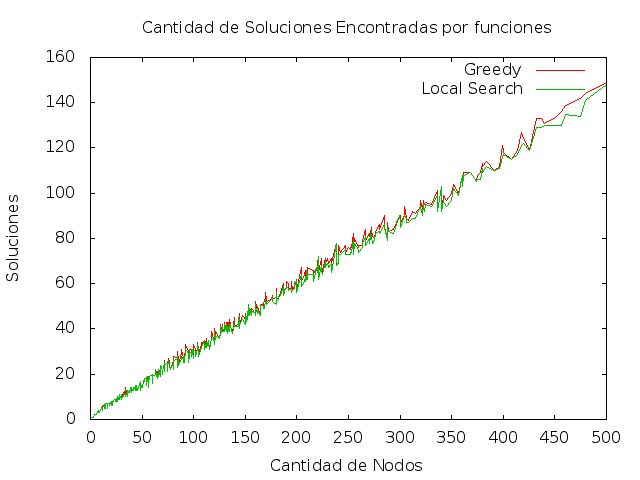
\includegraphics[width=17cm]{./graficos/comparacionSoluciones.png}
\end{center}

A efectos prácticos, y para el resto de las pruebas, utilizaremos como función de selección de los nodos a reemplazar e insertar a la función \textbf{DiffGrados}, que es la que selecciona como mejor candidato al que tenga menor diferencia entre los grados de los dos vértices a quitar y el grado del vértice a insertar.

\subsection{Mejor Caso}
Al igual que al algoritmo Greedy, pudimos verificar que nuestro algoritmo se comporta de forma optima para aquellos grafos que sean K-completos, los grafos bipartitos y para las distintas variantes de los arboles. Eso se debe a que, en todos los casos, no quedan nodos aislados a partir de las estrategias elegidas, y de ésta forma, la eliminación o el intercambio de nodos va trabajando con los mismos nodos con los que trabajaría el algoritmo exacto. \\
Cabe destacar que, para el caso del greedy sólo se es óptimo para los arboles binarios, cuando nuestro algoritmo de búsqueda local funcion óptimanete para todas sus variantes.\\
Además de éstos, que se comportan de la misma manera que el greedy, hemos encontrado una familia que es óptima para la heurística de búsqueda local, mejorando la solución obtenido por el algoritmo de greedy. Ésta familia se podría describir como los grafos en que el nodo de mayor grado no tiene ninguna conexión con los nodos hoja (es decir, sólo tiene un nodo adyacente). En el caso del greedy, el algoritmo tomaría al nodo que tiene mayor grado, por lo que además, debería tener en el CD a todos los nodos hoja. En cambio, nuestro algoritmo de busqueda local agarra esa solución no óptima, e intercambia y reemplaza nodos de forma tal de llegar a una solución óptima. \\

\begin{center}
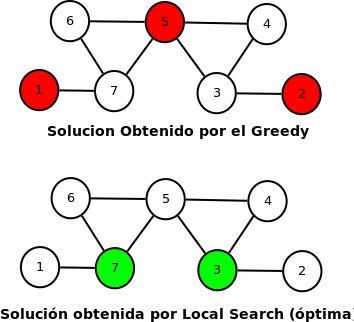
\includegraphics[width=8cm]{./graficos/familiaLocal.png}
\end{center}

En el ejemplo anterior, podemos ver un ejemplo de la familia mencionada anteriormente. El algoritmo greedy empezará por el nodo con mayor grado, y luego le quedarán 2 vértices con grado 1 en los extremos, por lo que tendrá que tomar a ambos. En cambio, la heurísitca de búsqueda local empezará de, por ejemplo, ésta solución de 3 nodos, y luego intercambiará los nodos con grado 1 por sus vecinos, para luego eliminar al nodo con mayor grado, quedando de ésta forma un conjunto dominante óptimo y de menor cardinalidad que la el greedy.

 \subsection{Peor Caso}
 Es claro que, al ser una heurística, en muchos casos la solución obtenida por la búsqueda local no es la óptima, pero de todas formas, se trata de soluciones cercanas a ella. En éste sentido, se dan cuando los nodos de la solución de la cual se parte la búsqueda local, tienen muchas aristas conectadas entre si o a otros vértices ya dominados (los grados de los nodos son muy altos). Ésto hace que, por ejemplo, las estrategias elegidas no puedan intercambiar nodos, o quitar nodos de la solución de la que se parta y, sin embargo, en la práctica si exista una solución con menor cantidad de nodos. \\
Siguiendo la línea de análisis del algoritmo greedy, pudimos ver que nuevamente la familia de los grafos Grid, con nuestro algoritmo de búsqueda local, no logra una solución óptima. Sin embargo, si hemos notado que, si le proporcionamos a nuestro algoritmo como solución inicial un CD obtenido con la heurística greedy, existen casos en que la cardinalidad se reduce en hasta 3 nodos, pero aún así la solución no logra ser la óptima. Es decir, para algunos casos particulares de grafos pertenecientes a ésta familia, logramos encontrar una solución levemente mejor a la inicial (greedy), pero aún así, podemos ubicar la familia dentro los casos en que no se llega a la solución óptima, al menos en hasta 29 nodos, que es la cantidad máxima que pudimos calcular con el algoritmo exacto. \\
Otra de las familias analizadas en la heurística greedy, la de los grafos de Mobius, está también dentro de ésta categoría en que el el algoritmo no nos proporciona la solución exacta. Pero, en ésta ocasión se diferencia con el Grid en que incluso no llega a mejor la solución inicial en ninguno de los casos estudiados. Más precisamente, corrimos el algoritmo con dos soluciones iniciales diferentes, para ver cuál éra su comportamiento. \\
En primer lugar, le dimos comos solución inicial (es decir, como conjunto dominante) a todos los vértices del grafo. Para esos casos, nuestra heurística, incluso, obtenía un conjunto dominante con mayor cantidad de nodos que los obtenidos por el algoritmo greedy. Y por otro lado, probamos como otra solución inicial al conjunto dominante que nos devolvía el algoritmo greedy, y en todos los casos, la cardinalidad del CD no pudo ser reducida (claro está, en casos en que la solución no era la óptima). Ésto se debe a que el algoritmo greedy nos da como solución inicial nodos 3-regulares, lo que hace que el algoritmo de búsqueda local tenga pocos vecinos en los que buscar y poder intercambiarse. Es por ello que podemos afirmar que para la familia de grafos de Mobius, nuestro algoritmo nunca logrará encontrar una solución óptima, con excepción de si el CD que se le pasó como solución inicial ya es óptimo. \\
Éstos resultados, eran de esperarse, ya que se trata de una heurísitca y sólo en algunos casos partículares (los mencionados en la sección Mejor Caso) se consiguen los mismos resultados que en los algoritmos exáctos. La idea, entonces, es intentar de construir las mejores estrategias para poder llegar a un resultado lo más exacto posible, para instancias en que sea imposible (al menos hoy en día) correr el algoritmo exácto, de orden exponencial. En éste caso particular, de la búsqueda local, seguramente haya muchas estrategias para mejorar o agregar, que nos aproximen a una solución un poco más exacta de la que encontramos hasta ahora, pero no pudimos dar con ellas en éste informe.


\subsection{Tests y análisis}
En primer lugar, y para acotar siempre la complejidad para el peor caso, en todos los gráficos que presentemos en ésta sección utilizaremos grafos de la familia de Mobius, por lo expuesto en la sección anterior respecto a su complejidad para el algoritmo de búsqueda local. Además, como comentamos también anteriormente, para ordenar los posibles nodos candidatos, utilizaremos la función de comparación \textbf{DiffGrados}.
Una vez establecida qué función deberíamos utilizar para el 2x1, nos abocamos a testear el método de búsqueda local de acuerdo a la cantidad de nodos del grafo y el tiempo que le consume encontrar una solución. Vale aclarar que no tomamos en consideración el tiempo que nos consume encontrar una solución para darle a la búsqueda local, ya que consideramos que ello no es parte de nuestro algoritmo. De ésta forma, podemos ver que nuestro algoritmo se comporta de forma polinómica en función del tiempo, como lo analizamos en la sección de complejidad. Es decir, mientras mayor cantidad de nodos tenga la solución que nos proveen, y más relacionados estén entre sí dichos nodos (es decir, a través de aristas hacia nodos del mismo conjunto o del conjunto de los dominados), mayor tiempo requerirá calcular nuestra solución. \\
El siguiente gráfico tiene como función mostrar la complejidad de nuestro algoritmo, que como dijimos tiene una complejidad de $O(n^4)$. El mismo muestra el tiempo que le toma a nuestro algoritmo encontrar la solucion, para grafos que parten desde 2 a 500 nodos. Como dijimos anteriormente, utilizamos grafos de la familia de Mobius. Además, se incluye en el gráfico la función $(1.05x^4)$, para mostrar que, aproximadamente, nuestro algoritmo se comporta de ésta manera.  \\
\begin{center}
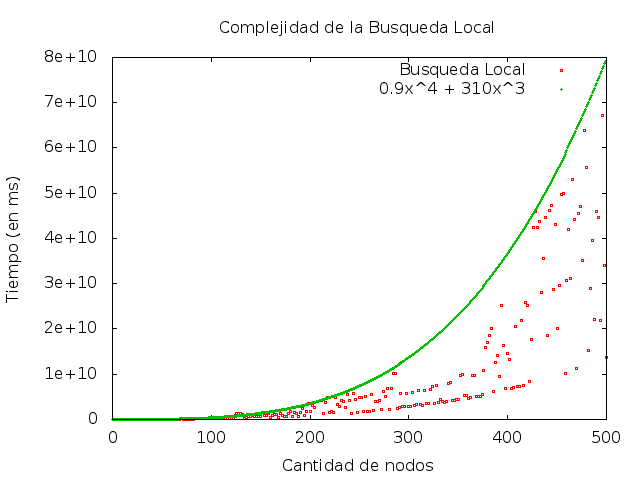
\includegraphics[width=17cm]{./graficos/complejidadLocal.png}
\end{center}

En el gráfico anterior podemos apreciar como nuestro algoritmo, a lo sumo, se comporta de de la misma forma que la función polinómica contra la que la comparamos. La dispersión de los puntos se debe a que, de acuerdo a la solución que se le pase al algoritmo y a la solución parcial que se esté construyendo, ésto modifica la performance del mismo. Vale la pena destacar que mientras que la estrategia del 2x1 tiene una complejidad de $O(n^4)$, las otras dos tienen una complejidad de $O(n^2)$, de forma tal que una solución que se construya a base de éstas dos últimas estrategias tendrá una complejidad menor a una que lo haga siempre reemplazando nodos por la estrategia del 2x1. Lo interesante entonces, es, analizar cómo crece el tiempo insumido por nuestro algoritmo a medida que se van agregando nodos al grafo, y se puede ver cómo crece de forma similar a la función estudiada. También podemos ver que hay algunos puntos, aislados, que están por arriba de la cota de la función mencionada, pero son sólo algunos pocos y son valores cercanos a la misma, por lo que la función encontrada es la que mejor se acerca al crecimiento de nuestro algoritmo. Cabe recordar que ésta función es una cota superior para los peores casos, por lo que es de esperar, como comentamos antes, que haya punto que una cantidad de nodos $(n)$ tenga valores bastante lejanos a los de la funcion en ese punto, pero lo interesante es mostrar que, a rasgos generales, el tiempo que se toma nuestro algoritmo aumenta de la misma forma que lo hace ésta función.\\
Por otro lado, como se puede apreciar, si bien el algoritmo es mucho mejor que el exacto en función de complejidad, tiene un orden de complejidad mayor que el algoritmo greedy. Además, ésto no nos asegura que la solución que encontramos sea la que efectivamente estamos buscando. En las próximas secciones estudiaremos más a fondo las relaciones entre la cantidad de soluciones encontradas y sus complejidades para las distintos algoritmos, para grafos generados al azar. La idea será determinar en qué situaciones conviene aplicar cual o tal técnica, si es que se puede determinar de antemano.
